% Provenance (never printed): see sources/outline_sources.md (Year 3: the main
% field and its secular variation, rock magnetism, palaeomagnetic poles, apparent
% polar wander, magnetostratigraphy, the geodynamo). Brief: sources/book5/BRIEFS.md,
% ch. 4. Curves and maps from figdata/bachelor-3/igrf_field.py (IGRF-14),
% palaeomag_stats.py (the invented Kesta terrane, its Fisher statistics, the
% Zijderveld specimen and the reference APW path), magnetostratigraphy.py.
% Exercise and problem values in the Book 5 scratch calculator calc/ch04.py.
\chapter{Geomagnetisme dan Paleomagnetisme}\label{ch:b3:palaeomagnetism}

Aliran basal yang meletus enam puluh juta tahun lalu mendingin dengan butir-butir kecil
magnetit yang terkunci sejajar dengan medan pada masa itu. Hari ini dibor, diorientasi
di tempatnya, diiris menjadi silinder-silinder kecil, dan dipanaskan
bertahap di dalam ruangan yang terlindung dari medan masa kini, ia tetap menyatakan seberapa jauh
dahulu berada dari kutub dan ke arah mana ia menghadap. Ribuan pengukuran serupa itu
dari setiap benua dan setiap umur telah mengungkap bagaimana benua-benua berpindah
sebelum dasar samudra yang merekam gerakan itu terbentuk, dan urutan
pembalikan medan melalui lapisan-lapisan suatu runtunan
sedimen. Bab ini menguraikan medan seperti keadaannya kini, bagaimana batuan merekamnya,
cara suatu arah diekstraksi dan dirata-ratakan, serta apa yang disampaikan kutub paleomagnetik
tentang gerak suatu lempeng.

\begin{recall}
Bumi sebagai magnet dan deklinasi magnetik dibahas dalam volume-volume sekolah
buku fisika; domain magnetik, histeresis, remanensi, dan suhu Curie dibahas dalam
volume Tahun 3 buku fisika; medan dipol magnetik dibahas dalam
volume Tahun 1 buku fisika. Pembalikan magnetik dan polaritas normal dan terbalik
telah dijumpai di kelas 11. Lingkaran besar dan segitiga bola didefinisikan dalam
volume Tahun 1, pada babnya tentang astronomi bola; kron polaritas, skala waktu
polaritas geomagnetik, anomali magnetik laut, dan rotasi berhingga
terhadap kutub Euler dalam babnya tentang kinematika lempeng pada bola;
jejak titik panas dalam babnya tentang titik panas. Harmonik bola dan
fungsi Legendre ternormalisasi Schmidt $P_n^m$ dipakai untuk gravitasi dalam
bab tentang gravitasi dan bentuk Bumi (lihat \cref{ch:b3:gravity-geodesy}).
\end{recall}

\section{Medan utama}

\begin{definition}[Medan geomagnetik utama; dipol aksial geosentris]\label{def:b3:palaeomagnetism:main-field}
Yang disebut \emph{medan geomagnetik utama}\index{medan geomagnetik utama} adalah bagian dari
medan magnet Bumi yang dihasilkan di dalam Bumi, yakni di inti luar
yang berupa besi cair; medan ini berubah dalam rentang tahun hingga jutaan tahun, tidak seperti
medan ionosfer dan magnetosfer, yang berubah dalam hitungan detik hingga hari. Sementara itu,
\emph{dipol aksial geosentris}\index{dipol aksial geosentris} adalah medan dipol magnet
yang diletakkan di pusat Bumi dan sejajar dengan sumbu rotasi,
menunjuk ke selatan, sehingga garis medannya keluar dari belahan bumi selatan dan
masuk ke belahan bumi utara.
\end{definition}

Di setiap titik permukaan, medan $\mathbf F$ adalah vektor. Ia dinyatakan
dalam kerangka lokal (gambar di bawah): $X$ menuju utara geografis, $Y$ menuju
timur, $Z$ ke bawah. Komponen horizontalnya adalah $H = \sqrt{X^2 + Y^2}$,
intensitas total $F = |\mathbf F|$, deklinasi magnetiknya $D$ adalah sudut dari
utara geografis ke $\mathbf H$, diukur searah jarum jam, dan inklinasinya $I$ adalah
sudut dari bidang horizontal ke $\mathbf F$.

\begin{definition}[Inklinasi magnetik]\label{def:b3:palaeomagnetism:inclination}
Yang disebut \emph{inklinasi magnetik}\index{inklinasi magnetik} $I$ medan di suatu
titik adalah sudut antara vektor medan dan bidang horizontal, positif jika medan
menunjuk ke bawah: $\tan I = Z/H$, dengan $-\ang{90} \le I
\le \ang{90}$.
\end{definition}

\begin{omfigure}
\begin{tikzpicture}[font=\small, x=1cm, y=1cm, >={Stealth[length=5pt]}]
% schematic; X = 3.0, Y = 1.0 (along the oblique east axis), Z = 2.4
\coordinate (O) at (0,0);
\coordinate (E) at (0.9,0.65);
\fill[gray!12] (-0.6,-0.43) -- (3.6,-0.43) -- ($(3.6,-0.43)+2.2*(E)$) -- ($(-0.6,-0.43)+2.2*(E)$) -- cycle;
\draw[->] (O) -- (4.0,0) node[right] {$X$, utara geografis};
\draw[->] (O) -- ($1.9*(E)$) node[above right] {$Y$, timur};
\draw[->] (O) -- (0,-3.0) node[below] {$Z$, bawah};
\coordinate (Hh) at ($(3.0,0)+1.0*(E)$);
\coordinate (F) at ($(Hh)+(0,-2.4)$);
\draw[densely dashed, gray] (3.0,0) -- (Hh);
\draw[densely dashed, gray] ($1.0*(E)$) -- (Hh);
\draw[densely dashed, gray] (Hh) -- (F);
\draw[densely dashed, gray] (0,-2.4) -- (F);
\draw[very thick, ->, blue!60!black] (O) -- (Hh) node[pos=0.3, above, sloped] {$\mathbf H$};
\draw[very thick, ->, red!70!black] (O) -- (F) node[pos=0.55, below left] {$\mathbf F$};
\draw[thick] (1.25,0) arc[start angle=0, end angle=9.46, radius=1.25];
\node at (1.62,0.13) {$D$};
\draw[thick, red!70!black] ($0.36*(Hh)$) to[bend left=30] ($0.3*(F)$);
\node[red!70!black] at (1.62,-0.42) {$I$};
\end{tikzpicture}

\par\smallskip{\small Unsur-unsur medan di suatu titik: komponen utara $X$, timur
$Y$, dan bawah $Z$, komponen horizontal $\mathbf H$, medan total
$\mathbf F$, deklinasi magnetik $D$ (pada bidang horizontal, abu-abu)
dan inklinasi $I$ (pada bidang vertikal yang memuat $\mathbf
F$).}\label{fig:b3:palaeomagnetism:elements}
\end{omfigure}

\begin{theorem}[Rumus dipol]\label{thm:b3:palaeomagnetism:dipole}
Pada permukaan bola berjari-jari $a$, medan \omterm{def:b3:palaeomagnetism:main-field}{dipol aksial geosentris}
dengan momen $m$ memiliki, pada lintang $\lambda$,
\[
  H = B_0\cos\lambda,\qquad Z = 2B_0\sin\lambda,\qquad
  F = B_0\sqrt{1 + 3\sin^2\lambda},\qquad
  \tan I = 2\tan\lambda,\qquad D = 0,
\]
dengan $B_0 = \mu_0 m/(4\pi a^3)$ adalah medan di khatulistiwa. Inilah
\emph{rumus dipol}\index{rumus dipol}.
\end{theorem}

\begin{proof}
Di luar sumbernya, medan diturunkan dari potensial skalar magnetik,
$\mathbf B = -\nabla V$. Untuk dipol dengan momen $m$ yang menunjuk sepanjang $-z$,
yakni selatan geografis, $V = -\mu_0 m\cos\theta/(4\pi r^2)$, dengan $\theta$ adalah
kolatitud. Dalam koordinat bola, $B_r = -\partial V/\partial r =
-2\mu_0 m\cos\theta/(4\pi r^3)$ dan $B_\theta = -(1/r)\,\partial V/\partial\theta =
-\mu_0 m\sin\theta/(4\pi r^3)$, dan $B_\varphi = 0$. Pada $r = a$, komponen ke bawah
adalah $Z = -B_r = 2B_0\cos\theta = 2B_0\sin\lambda$, dan karena
$\mathbf e_\theta$ menunjuk ke selatan, komponen ke utara adalah $X = -B_\theta =
B_0\sin\theta = B_0\cos\lambda$, dengan $Y = 0$. Maka $H = X$, $D = 0$, $\tan I =
Z/H = 2\tan\lambda$ dan $F^2 = B_0^2(\cos^2\lambda + 4\sin^2\lambda) =
B_0^2(1 + 3\sin^2\lambda)$.
\end{proof}

Inklinasi bernilai nol di khatulistiwa, \ang{90} di Kutub Utara, dan
negatif di belahan bumi selatan; intensitas di kutub dua kali lebih besar
daripada di khatulistiwa. Medan sebenarnya bukan dipol sempurna, dan
medan itu dijelaskan, seperti gravitasi, dengan harmonik bola.

\begin{definition}[Medan Referensi Geomagnetik Internasional]\label{def:b3:palaeomagnetism:igrf}
Yang disebut \emph{medan referensi geomagnetik internasional}\index{medan referensi geomagnetik internasional}
(IGRF) adalah model yang disepakati secara internasional untuk
medan utama: potensial, di permukaan dan di atasnya,
\[
  V(r,\theta,\varphi) = a\sum_{n=1}^{N}\Bigl(\frac ar\Bigr)^{n+1}\sum_{m=0}^{n}
  \bigl(g_n^m\cos m\varphi + h_n^m\sin m\varphi\bigr)P_n^m(\cos\theta),
\]
dengan $a = \qty{6371.2}{km}$, $\mathbf B = -\nabla V$, dan koefisien Gauss
$g_n^m$, $h_n^m$ (dalam \unit{nT}) yang diberikan setiap lima tahun sejak 1900,
bersama laju perubahannya selama lima tahun berikutnya.
\end{definition}
% ledger: geomag5:igrf, data:b5-igrf

Model ini dikelola oleh International Association of Geomagnetism and
Aeronomy; generasi keempat belasnya selesai pada November 2024 dan
dipotong pada derajat $N = 13$. Suku pertama, $g_1^0$, adalah dipol aksial:
dengan membandingkan pembuktian di atas, $B_0 = -g_1^0$, dan $g_1^0 = \qty{-29350}{nT}$
pada 2025. Dengan dua suku derajat-1 lainnya, dipol itu miring; sumbunya memotong
permukaan di kutub geomagnetik utara, di \ang{80.79}\,LU, \ang{72.76}\,BB pada
2025, dan momennya adalah $m = 4\pi a^3\sqrt{(g_1^0)^2 + (g_1^1)^2 +
(h_1^1)^2}/\mu_0 = \qty{7.69e22}{A.m^2}$.
% ledger: data:b5-igrf

\begin{omfigure}
\begin{tikzpicture}
\begin{groupplot}[group style={group size=1 by 2, vertical sep=1.4cm},
  ommap, width=0.96\linewidth, xtick={-180,-120,...,180}, ytick={-60,0,60},
  unbounded coords=jump, title style={font=\small, yshift=-1ex}]
\nextgroupplot[title={(a) inklinasi, setiap \ang{20}}]
% computed in figdata/bachelor-3/igrf_field.py; ledger: data:b5-igrf, data:ne-land
\addplot[fill=omLithAlluv, draw=black!45, line width=0.2pt, forget plot] table {figdata/out/shared-geo-land.dat};
\addplot[red!70!black, line width=0.5pt] table[x=x, y=y] {figdata/out/bachelor-3-igrf_field-incl.dat};
\addplot[black, line width=1.1pt] table[x=x, y=y] {figdata/out/bachelor-3-igrf_field-dipeq.dat};
\addplot[draw=none, nodes near coords, point meta=explicit,
  every node near coord/.style={font=\tiny, fill=white, inner sep=0.6pt, anchor=center}]
  table[x=x, y=y, meta=lev] {figdata/out/bachelor-3-igrf_field-inclab.dat};
\nextgroupplot[title={(b) intensitas total, setiap \qty{5000}{nT}}]
\addplot[fill=omLithAlluv, draw=black!45, line width=0.2pt, forget plot] table {figdata/out/shared-geo-land.dat};
\addplot[blue!60!black, line width=0.5pt] table[x=x, y=y] {figdata/out/bachelor-3-igrf_field-intens.dat};
\addplot[draw=none, nodes near coords, point meta=explicit,
  every node near coord/.style={font=\tiny, fill=white, inner sep=0.6pt, anchor=center}]
  table[x=x, y=y, meta=lev] {figdata/out/bachelor-3-igrf_field-intlab.dat};
\addplot[only marks, mark=x, mark size=3pt, line width=1pt, black] table {figdata/out/bachelor-3-igrf_field-fmin.dat};
\end{groupplot}
\end{tikzpicture}

\par\smallskip{\small Medan utama pada 2025 dari IGRF keempat belas, di
permukaan bola berjari-jari \qty{6371.2}{km}. (a) Inklinasi dalam derajat;
garis tebal, $I = 0$, adalah khatulistiwa kemiringan. (b) Intensitas total dalam \unit{nT};
tanda silang menandai medan terlemah, sekitar \qty{22100}{nT}, di atas
Atlantik Selatan, dibandingkan sekitar \qty{66600}{nT} di titik terkuat, di selatan
Australia.}\label{fig:b3:palaeomagnetism:igrf-maps}
\end{omfigure}

Peta di atas memperlihatkan seberapa jauh medan menyimpang dari dipol. Khatulistiwa kemiringan
menjauh hingga sekitar \ang{12} dari khatulistiwa geografis, dan intensitasnya,
yang pada dipol akan seragam sepanjang paralel, bervariasi dengan faktor
tiga, dengan minimum luas di atas Atlantik Selatan.
% ledger: data:b5-igrf

\begin{definition}[Variasi sekuler]\label{def:b3:palaeomagnetism:secular}
Yang disebut \emph{variasi sekuler}\index{variasi sekuler} adalah perubahan lambat dari
medan utama terhadap waktu, dalam rentang tahun hingga abad, diukur dengan laju perubahan
koefisien Gauss-nya atau unsur-unsurnya di suatu tempat.
\end{definition}

Selama 125 tahun terakhir, momen dipol turun dari
\qty{8.32e22}{A.m^2} menjadi \qty{7.69e22}{A.m^2}, sebesar \qty{7.6}{\percent}, dan
kutub geomagnetik utara telah bergeser dari \ang{78.61}\,LU, \ang{68.79}\,BB ke
posisinya sekarang (gambar di bawah); $g_1^0$ masih bertambah \qty{12.6}{nT} per tahun,
yakni melemahnya dipol.
% ledger: data:b5-igrf

\begin{omfigure}
\begin{tikzpicture}
\begin{groupplot}[group style={group size=2 by 1, horizontal sep=1.7cm},
  omrecord, width=0.47\linewidth, height=0.4\linewidth, xmin=1895, xmax=2030,
  xtick={1900,1950,2000}, xticklabel style={/pgf/number format/1000 sep=},
  xlabel={tahun}]
\nextgroupplot[ylabel={momen dipol (\qty{e22}{A.m^2})}, ymin=7.6, ymax=8.4]
% computed in figdata/bachelor-3/igrf_field.py; ledger: data:b5-igrf
\addplot[omDef, thick, mark=*, mark size=1pt] table[x=year, y=M] {figdata/out/bachelor-3-igrf_field-dipole.dat};
\nextgroupplot[ylabel={lintang kutub (\unit{\degree}\,LU)}, ymin=78, ymax=81.5]
\addplot[red!70!black, thick, mark=*, mark size=1pt] table[x=year, y=plat] {figdata/out/bachelor-3-igrf_field-dipole.dat};
\end{groupplot}
\end{tikzpicture}

\par\smallskip{\small Bagian dipol dari medan utama, 1900--2025, setiap lima
tahun, dari IGRF: momennya (kiri) dan lintang dari
kutub geomagnetik utara (kanan).}\label{fig:b3:palaeomagnetism:dipole}
\end{omfigure}

Dari mana medan itu berasal? Magnet permanen dapat dikesampingkan: suhu Curie
magnetit sekitar \qty{580}{\celsius} dan hematit
\qty{675}{\celsius}, dan Bumi bagian dalam jauh lebih panas. Medan ini
diperbarui terus-menerus oleh gerakan cairan konduktif
di inti luar.
% ledger: tarduno:curie

\begin{definition}[Geodinamo]\label{def:b3:palaeomagnetism:geodynamo}
Yang disebut \emph{geodinamo}\index{geodinamo} adalah proses yang berlangsung sendiri melalui
konveksi cairan paduan besi konduktif listrik di inti luar,
yang dibelokkan oleh rotasi Bumi, menginduksi arus listrik yang medan magnetnya
mempertahankan dirinya terhadap peluruhan ohmik.
\end{definition}

\begin{proposition}[Persamaan induksi]\label{prop:b3:palaeomagnetism:induction}
Dalam konduktor dengan difusivitas magnetik $\eta = 1/(\mu_0\sigma)$ yang bergerak dengan
kecepatan $\mathbf u$, medan magnet memenuhi
\[
  \frac{\partial\mathbf B}{\partial t} = \nabla\times(\mathbf u\times\mathbf B)
  + \eta\nabla^2\mathbf B .
\]
\end{proposition}
\admitted

Suku pertama meregangkan dan memuntir garis medan yang dibawa oleh aliran; suku
kedua membuat medan meluruh, dalam benda berukuran $L$, dalam waktu berorde
$L^2/\eta$. Dinamo bekerja apabila aliran membangkitkan kembali medan lebih cepat
daripada medan itu berdifusi menjauh. Simulasi komputer cangkang fluida yang
berkonveksi dan berotasi mereproduksi dipol aksial dominan dan, sesekali, suatu pembalikan; namun
persamaan \omterm{def:b3:palaeomagnetism:geodynamo}{geodinamo}, yang digandengkan dengan persamaan aliran, berada di luar
buku ini. Selain pembalikan penuh, catatan juga memuat peristiwa yang lebih singkat.

\begin{definition}[Ekskursi geomagnetik]\label{def:b3:palaeomagnetism:excursion}
Yang disebut \emph{ekskursi geomagnetik}\index{ekskursi geomagnetik} adalah penyimpangan besar
  arah medan dari arah dipol aksial, dengan
\omterm{def:b3:palaeomagnetism:vgp}{kutub geomagnetik virtual} (\cref{def:b3:palaeomagnetism:vgp}) bergerak jauh dari
kutub geografis, yang kembali ke polaritas semula alih-alih
menyelesaikan suatu pembalikan.
\end{definition}

\section{Bagaimana batuan merekam medan}

Mineral feromagnetik dalam arti luas, terutama magnetit pada batuan beku
dan hematit pada sedimen merah, membawa remanensi. Di atas suhu Curie-nya,
sebutir tidak memilikinya; di bawah suhu itu, butir kecil merupakan satu domain magnetik tunggal yang
momennya berbalik di antara arah-arah mudahnya, secara termal teraktivasi, setelah
waktu relaksasi
\[
  \tau = \frac1C\exp\Bigl(\frac{K V}{k_B T}\Bigr),
\]
dengan $K$ adalah energi anisotropi per satuan volume, $V$ volume butir
dan $C$ faktor frekuensi. Ini adalah hukum relaksasi Néel, yang di sini diterima tanpa bukti. Karena
$\tau$ tumbuh secara eksponensial saat $T$ turun, sebutir melintasi rentang
suhu yang sempit dari berbalik bebas hingga mempertahankan momennya selama miliaran
tahun.

\begin{definition}[Suhu pemblokiran]\label{def:b3:palaeomagnetism:blocking}
Yang disebut \emph{suhu pemblokiran}\index{suhu pemblokiran} suatu butir magnetik
adalah suhu yang di bawahnya waktu relaksasinya melampaui waktu
percobaan, sehingga momennya tetap: saat mendingin melewatinya, butir merekam
medan; saat dipanaskan melewatinya dalam medan nol, butir kehilangan
rekaman itu.
\end{definition}

\begin{definition}[Magnetisasi remanen alami, termal, detrital dan kimia]\label{def:b3:palaeomagnetism:nrm}
Yang disebut \emph{magnetisasi remanen alami}\index{magnetisasi remanen alami}
(NRM) suatu batuan adalah remanensi yang dibawanya saat dikumpulkan, yakni jumlah dari
komponen yang diperoleh pada waktu-waktu berbeda. Yang disebut \emph{magnetisasi
termoremanen}\index{magnetisasi termoremanen} (TRM) diperoleh dengan mendingin
melewati \omterm{def:b3:palaeomagnetism:blocking}{suhu pemblokiran} dalam suatu medan, seperti pada aliran lava atau
intrusi. Yang disebut \emph{magnetisasi remanen detrital}\index{magnetisasi remanen detrital}
(DRM) diperoleh ketika butir magnetik mengendap dalam air, atau dalam
sedimen basah tepat di bawah permukaannya, berotasi ke arah medan sebelum
terkunci. Yang disebut \emph{magnetisasi remanen kimia}\index{magnetisasi remanen kimia}
(CRM) diperoleh ketika suatu mineral magnetik tumbuh, melalui
volume pemblokiran, dalam suatu medan, seperti hematit saat lapisan merah terbentuk.
\end{definition}

TRM merekam medan pada saat pendinginan; DRM, dalam waktu yang
diperlukan sedimen untuk memadat; CRM, kapan pun mineralnya tumbuh, yang bisa jauh
setelah pengendapan. Pemanasan kemudian, atau medan sekarang yang bekerja dalam waktu lama
pada butir dengan waktu relaksasi singkat, menambahkan komponen sekunder di atasnya:
remanensi viskos searah medan terkini.

\section{Dari spesimen ke arah}

Inti terorientasi dibor di beberapa lokasi dalam suatu formasi, beberapa inti per
lokasi, dan dipotong menjadi spesimen berukuran beberapa sentimeter kubik. NRM tiap
spesimen diukur, lalu dihilangkan secara bertahap.

\begin{definition}[Demagnetisasi bertahap]\label{def:b3:palaeomagnetism:demag}
Yang disebut \emph{demagnetisasi bertahap}\index{demagnetisasi bertahap} adalah penghilangan
remanensi suatu spesimen dalam langkah-langkah intensitas yang meningkat, sambil mengukur
vektor sisa setelah tiap langkah: dengan memanaskan hingga suhu yang makin tinggi lalu
mendinginkannya dalam medan nol (demagnetisasi termal), yang menghilangkan komponen dengan
\omterm{def:b3:palaeomagnetism:blocking}{suhu pemblokiran} lebih rendah lebih dulu, atau dengan medan magnet bolak-balik yang meningkat
berpuncak lalu meluruh ke nol (demagnetisasi medan bolak-balik), yang menghilangkan
komponen dengan koersivitas lebih rendah lebih dulu.
\end{definition}

\begin{definition}[Diagram Zijderveld; magnetisasi remanen karakteristik]\label{def:b3:palaeomagnetism:zijderveld}
Yang disebut \emph{diagram Zijderveld}\index{diagram Zijderveld} menggambarkan titik-titik ujung
vektor remanensi sisa setelah tiap langkah demagnetisasi pada dua bidang
sekaligus, yaitu horizontal (utara terhadap timur) dan satu bidang vertikal (utara
terhadap bawah), dengan sumbu utara yang sama. Suatu komponen yang dihilangkan sendirian selama rentang
langkah tergambar sebagai ruas garis lurus; ruas yang berakhir di titik asal adalah
\emph{magnetisasi remanen karakteristik}\index{magnetisasi remanen karakteristik}
(ChRM), komponen yang paling stabil, yang ditafsirkan sebagai komponen primer
bila uji memungkinkan.
\end{definition}

Spesimen pada gambar di bawah memuat dua komponen: timpaan viskos
searah medan sekarang, yang hilang pada \qty{300}{\celsius}, dan ChRM
terlepas dari 300 hingga \qty{580}{\celsius}, yaitu suhu Curie magnetit.
Di atas \qty{300}{\celsius} kedua proyeksi berjalan lurus ke titik asal; arah
ruas itu adalah ChRM.

\begin{omfigure}
\begin{tikzpicture}
\begin{groupplot}[group style={group size=2 by 1, horizontal sep=1.3cm},
  width=0.5\linewidth]
\nextgroupplot[axis lines=middle, axis equal image, xmin=-4, xmax=36, ymin=-4, ymax=42,
  y dir=reverse, xlabel={U}, ylabel={T, bawah}, tick label style={font=\scriptsize},
  xtick={0,10,20,30}, ytick={10,20,30,40}, label style={font=\small},
  xlabel style={at={(ticklabel* cs:1.0)}, anchor=west},
  ylabel style={at={(ticklabel* cs:1.0)}, anchor=north west},
  title={(a) Diagram Zijderveld (\unit{mA/m})}, title style={font=\small, yshift=1ex},
  clip=false, legend style={font=\scriptsize, at={(0.13,0.03)}, anchor=south west, cells={anchor=west}}]
% computed in figdata/bachelor-3/palaeomag_stats.py (synthetic specimen)
\addplot[black, mark=*, mark size=1.5pt] table[x=N, y=E] {figdata/out/bachelor-3-palaeomag_stats-zij.dat};
\addlegendentry{horizontal: U, T}
\addplot[black, mark=o, mark size=1.7pt, fill=white] table[x=N, y=Down] {figdata/out/bachelor-3-palaeomag_stats-zij.dat};
\addlegendentry{vertikal: U, bawah}
\node[font=\scriptsize, anchor=south west] at (axis cs:32.2,18.1) {\qty{20}{\celsius}};
\node[font=\scriptsize, anchor=north west] at (axis cs:32.2,38.2) {\qty{20}{\celsius}};
\node[font=\scriptsize, anchor=south] at (axis cs:25.8,17.6) {300};
\node[font=\scriptsize, anchor=east] at (axis cs:25.0,24.6) {300};
\node[font=\scriptsize, anchor=south east] at (axis cs:-0.5,-0.5) {580};
\nextgroupplot[axis equal image, hide axis, clip=false, xmin=-1.12, xmax=1.12, ymin=-1.12, ymax=1.18,
  title={(b) situs A, proyeksi sama luas, belahan bawah}, title style={font=\small, yshift=1ex}]
\addplot[black, domain=0:360, samples=145, thin] ({cos(x)},{sin(x)});
\draw[black] (axis cs:0,1) -- (axis cs:0,1.08) node[above, font=\scriptsize] {U};
\draw[black] (axis cs:1,0) -- (axis cs:1.06,0);
\draw[black] (axis cs:0,-1) -- (axis cs:0,-1.06);
\draw[black] (axis cs:-1,0) -- (axis cs:-1.06,0);
\draw[black] (axis cs:-0.04,0) -- (axis cs:0.04,0) (axis cs:0,-0.04) -- (axis cs:0,0.04);
\addplot[only marks, mark=*, mark size=1.6pt, black] table[x=x, y=y] {figdata/out/bachelor-3-palaeomag_stats-dirsA.dat};
\addplot[omDef, thick] table[x=x, y=y] {figdata/out/bachelor-3-palaeomag_stats-cone.dat};
\addplot[only marks, mark=star, mark size=3.5pt, omDef, line width=0.9pt] table[x=x, y=y] {figdata/out/bachelor-3-palaeomag_stats-meanA.dat};
\end{groupplot}
\end{tikzpicture}

\par\smallskip{\small (a) Demagnetisasi termal sebuah spesimen sintetis, dari
\qty{20}{\celsius} sampai \qty{580}{\celsius}: titik terisi, proyeksi
horizontal; titik terbuka, proyeksi vertikal. (b) Keenam arah ChRM dari situs A
soal akhir pekan (titik), rata-ratanya (bintang) dan kerucut
keyakinan 95 persennya (lingkaran).}\label{fig:b3:palaeomagnetism:zijderveld}
\end{omfigure}

Arah-arah spesimen pada suatu situs menyebar di sekitar rata-rata, dan
statistik penyebaran itu adalah statistik suatu distribusi pada bola.

\begin{proposition}[Distribusi Fisher]\label{prop:b3:palaeomagnetism:fisher}
Yang disebut \emph{distribusi Fisher}\index{distribusi Fisher} dengan parameter presisi
$\kappa > 0$ terhadap arah rata-rata memberikan vektor satuan massa jenis peluang
per satuan sudut ruang,
\[
  f(\theta) = \frac{\kappa}{4\pi\sinh\kappa}\,e^{\kappa\cos\theta},
\]
dengan $\theta$ adalah sudutnya terhadap rata-rata. Diberikan $N$ vektor satuan $\mathbf u_i$
yang diambil darinya, dengan resultan $\mathbf R = \sum\mathbf u_i$ berpanjang $R$, taksiran
terbaik arah rata-rata adalah arah $\mathbf R$; presisinya
ditaksir oleh $k = (N - 1)/(N - R)$; dan rata-rata sebenarnya terletak, dengan peluang
$1 - p$, dalam sudut $\alpha_{1-p}$ dari rata-rata taksiran, dengan
\[
  \cos\alpha_{1-p} = 1 - \frac{N - R}{R}\Bigl[\Bigl(\frac1p\Bigr)^{1/(N-1)} - 1\Bigr].
\]
\end{proposition}
\admitted

\begin{definition}[Alfa-95]\label{def:b3:palaeomagnetism:a95}
Yang disebut \emph{alfa-95}\index{alfa-95} ($\alpha_{95}$) dari suatu arah rata-rata adalah
semi-sudut kerucut keyakinan 95 persennya, yaitu sudut $\alpha_{1-p}$ pada
\cref{prop:b3:palaeomagnetism:fisher} untuk $p = 0.05$.
\end{definition}

Massa jenis peluang itu berintegral satu: dengan $\mathrm d\Omega = 2\pi\sin\theta\,\mathrm
d\theta$, $\int_0^\pi f\,2\pi\sin\theta\,\mathrm d\theta =
\frac{\kappa}{2\sinh\kappa}\cdot\frac{e^\kappa - e^{-\kappa}}{\kappa} = 1$. Arah-arah dirata-ratakan sebagai
vektor satuan, bukan sebagai sudut: rata-rata deklinasi \ang{350} dan \ang{10} adalah
utara, bukan selatan. Nilai $k$ yang besar berarti gerombolan yang rapat, dan $\alpha_{95}$ mengecil
kira-kira sebanding dengan $1/\sqrt{kN}$.

\begin{method}[Uji lapangan arah paleomagnetik]\label{met:b3:palaeomagnetism:tests}
ChRM dapat ditunjukkan lebih tua daripada suatu peristiwa melalui uji yang dilakukan di lapangan.
\begin{itemize}
  \item \textbf{Uji lipatan.} Situs pada kedua sayap suatu lipatan: jika arah-arahnya
        lebih mengelompok setelah lapisan diputar kembali ke horizontal daripada
        sebelumnya, magnetisasinya lebih tua daripada pelipatan.
  \item \textbf{Uji pembalikan.} Jika suatu formasi memuat kedua polaritas, rata-rata
        arah terbalik, setelah dibalik, seharusnya berimpit dengan rata-rata
        arah normal dalam kerucut keyakinannya masing-masing; tumpang-tindih viskos yang tidak
        dihilangkan akan membias keduanya ke arah yang sama dan merusak antipodalitas.
  \item \textbf{Uji kontak terpanggang.} Retas memanaskan batuan induk di sebelahnya,
        yang memperoleh TRM baru: jika batuan yang terpanggang membawa arah retas dan
        batuan induk yang lebih jauh membawa arah yang berbeda, magnetisasi retas
        belum direset sejak ia mendingin.
\end{itemize}
\end{method}

\section{Kutub dan lempeng}

Jika medan, dirata-ratakan selama beberapa ribu tahun untuk meredam
\omterm{def:b3:palaeomagnetism:secular}{variasi sekuler}, merupakan \omterm{def:b3:palaeomagnetism:main-field}{dipol aksial geosentris}, maka \omterm{thm:b3:palaeomagnetism:dipole}{rumus dipol} mengubah inklinasi rata-rata
menjadi lintang, dan deklinasi rata-rata menunjuk ke kutub.

\begin{definition}[Paleolintang; kutub geomagnetik virtual]\label{def:b3:palaeomagnetism:vgp}
Yang disebut \emph{paleolintang}\index{paleolintang} suatu situs adalah lintang
$\lambda$ yang diberikan oleh inklinasi rata-ratanya melalui \omterm{thm:b3:palaeomagnetism:dipole}{rumus dipol}, $\tan I =
2\tan\lambda$. \emph{Kutub geomagnetik virtual}\index{kutub geomagnetik virtual}
(VGP) dari arah $(D, I)$ yang diamati di suatu situs adalah kutub utara
dipol geosentris yang akan menghasilkan arah itu di sana.
\end{definition}

\begin{theorem}[Kutub dari suatu arah]\label{thm:b3:palaeomagnetism:pole}
Misalkan suatu situs memiliki lintang $\lambda_s$ dan bujur $\varphi_s$ serta
arah rata-rata $(D, I)$. Misalkan $p$ adalah paleokolatitud, $\cot p = \tfrac12\tan I$,
dengan $0 \le p \le \ang{180}$. \omterm{def:b3:palaeomagnetism:vgp}{Kutub geomagnetik virtual} memiliki lintang
$\lambda_p$ dan bujur $\varphi_p$ yang diberikan oleh
\[
  \sin\lambda_p = \sin\lambda_s\cos p + \cos\lambda_s\sin p\cos D,\qquad
  \sin\beta = \frac{\sin p\sin D}{\cos\lambda_p},
\]
dengan $\varphi_p = \varphi_s + \beta$ jika $\cos p \ge \sin\lambda_s\sin\lambda_p$,
dan $\varphi_p = \varphi_s + \ang{180} - \beta$ jika tidak.
\end{theorem}

\begin{proof}
Pada bola, situs $S$, kutub utara geografis $N$, dan VGP $P$ membentuk
segitiga bola (gambar di bawah). Sisi $NS$ adalah kolatitud situs,
$\ang{90} - \lambda_s$; sisi $SP$ adalah jarak sudut dari situs ke
kutub dipol, yang oleh \omterm{thm:b3:palaeomagnetism:dipole}{rumus dipol} diberikan sebagai $p$, karena lintang magnetik situs
adalah $\ang{90} - p$; dan sudut di $S$, antara arah ke $N$ dan
arah ke $P$, adalah deklinasi $D$. Aturan kosinus untuk
sisi $NP = \ang{90} - \lambda_p$ memberikan relasi pertama; aturan sinus,
$\sin\beta/\sin p = \sin D/\sin(\ang{90} - \lambda_p)$, memberikan sudut $\beta$
di $N$, yaitu selisih bujur. Sinus hanya menentukan $\beta$ sampai
suplemennya: aturan kosinus untuk sisi $SP$, $\cos p = \sin\lambda_s
\sin\lambda_p + \cos\lambda_s\cos\lambda_p\cos\beta$, menunjukkan bahwa $\cos\beta \ge
0$ tepat ketika $\cos p \ge \sin\lambda_s\sin\lambda_p$.
\end{proof}

\begin{omfigure}
\begin{tikzpicture}[font=\small, >={Stealth[length=5pt]}]
\draw[gray!60] (0,0) circle (2.6);
\draw[gray!50, densely dashed] (-2.6,0) arc[start angle=180, end angle=360, x radius=2.6, y radius=0.7];
\coordinate (N) at (0,2.6);
\coordinate (S) at (-1.2,0.25);
\coordinate (P) at (1.25,1.65);
\fill (N) circle (1.6pt) node[above] {$N$};
\fill (S) circle (1.6pt) node[below left] {$S$ (situs)};
\fill[omDef] (P) circle (1.8pt) node[right] {$P$ (VGP)};
\draw[thick] (N) to[bend right=12] node[left, pos=0.55] {$\ang{90}-\lambda_s$} (S);
\draw[thick, omDef] (S) to[bend left=10] node[below right, pos=0.55] {$p$} (P);
\draw[thick, blue!60!black] (N) to[bend left=12] node[above right, pos=0.45] {$\ang{90}-\lambda_p$} (P);
\draw ($(S)!0.2!(N)$) to[bend left=35] ($(S)!0.2!(P)$);
\node[inner sep=1pt] at (-0.61,0.86) {$D$};
\draw ($(N)!0.18!(S)$) to[bend right=40] node[below, pos=0.5, inner sep=2pt] {$\beta$} ($(N)!0.18!(P)$);
\end{tikzpicture}

\par\smallskip{\small Segitiga bola dari \omterm{def:b3:palaeomagnetism:vgp}{kutub geomagnetik virtual}:
kutub utara geografis $N$, situs $S$, kutub $P$. Sudut di situs adalah
deklinasi $D$; sudut di kutub $N$ adalah selisih bujur
$\beta$.}\label{fig:b3:palaeomagnetism:vgp}
\end{omfigure}

Kerucut $\alpha_{95}$ di sekitar arah rata-rata menjadi lonjong di sekitar kutub,
dengan semi-sumbu $\mathrm dp = \tfrac12\alpha_{95}(1 + 3\cos^2p)$ sepanjang lingkaran besar
dari situs, dan $\mathrm dm = \alpha_{95}\sin p/\cos I$ melintang terhadapnya. Kutub
yang dirata-ratakan dari beberapa situs suatu formasi, masing-masing berupa VGP, adalah kutub paleomagnetik
dengan kerucutnya sendiri, $A_{95}$. Batuan dengan umur yang sama pada satu lempeng kaku memberikan
kutub yang sama; batuan dengan umur berbeda, kutub yang berbeda.

\begin{definition}[Pengembaraan kutub semu; lintasan pengembaraan kutub semu]\label{def:b3:palaeomagnetism:apw}
\emph{Pengembaraan kutub semu}\index{pengembaraan kutub semu} adalah perubahan, seiring
dengan umur batuan, dari kutub paleomagnetik suatu lempeng yang dilihat dari lempeng itu,
dengan lempeng itu dianggap tetap. \emph{Lintasan pengembaraan kutub semu}\index{lintasan pengembaraan kutub semu}
adalah kurva yang menghubungkan kutub-kutub paleomagnetik suatu lempeng secara berurutan
menurut umur.
\end{definition}

Kutub itu sendiri tidak mengembara: lempenglah yang bergerak, dan lintasan itu mencatat
gerak tersebut secara terbalik. Dua lempeng yang telah saling menjauh memiliki lintasan yang berbeda untuk kurun waktu
sebelum pemisahan mereka, dan tiap lintasan diputar agar berimpit dengan yang lain oleh
rotasi berhingga yang menutup samudra di antara keduanya. Kutub paleomagnetik menetapkan
lintang suatu blok dan orientasinya, tetapi tidak bujurnya: rotasi
blok terhadap sumbu rotasi tidak mengubah keduanya.

Blok yang berpindah, yakni terrane, diuji terhadap lintasan lempeng stabil tempat ia
kini menjadi bagian. Dari kutub acuan dengan umur yang tepat dihitung arah yang diharapkan
$(D_x, I_x)$ di situs, dengan \cref{thm:b3:palaeomagnetism:pole}
dibaca mundur. Rotasi searah jarum jam blok terhadap sumbu vertikal adalah
diukur dengan $R = D_o - D_x$, dan perpindahan ke arah kutubnya dengan $P = \lambda_x -
\lambda_o$, yaitu selisih antara \omterm{def:b3:palaeomagnetism:vgp}{paleolintang} yang diharapkan dan yang diamati; galat
deklinasi kira-kira $\Delta D = \arcsin(\sin\alpha_{95}/\cos I)$,
dan galat-galat digabungkan sebagai akar jumlah kuadratnya. Rantai
Hawaii--Emperor diuji seperti ini pada volume Tahun 1, dalam bab tentang titik panas:
\omterm{def:b3:palaeomagnetism:vgp}{paleolintang} yang diukur pada gunung laut Emperor memperlihatkan titik panas itu sendiri
bergerak ke selatan, lebih dari \qty{40}{mm/yr} dari 81 sampai \qty{47}{Ma}.
% ledger: tarduno:emperor

\begin{omfigure}
\begin{tikzpicture}
\begin{axis}[axis equal image, hide axis, width=0.62\linewidth,
  xmin=-0.62, xmax=0.62, ymin=-0.62, ymax=0.62, unbounded coords=jump,
  legend style={font=\scriptsize, at={(1.03,0.5)}, anchor=west, cells={anchor=west}}]
% computed in figdata/bachelor-3/palaeomag_stats.py (invented continent and terrane)
\addplot[gray!50, line width=0.3pt, forget plot] table[x=x, y=y] {figdata/out/bachelor-3-palaeomag_stats-graticule.dat};
\addplot[black, line width=0.6pt, domain=0:360, samples=145, forget plot]
  ({0.5412*cos(x)},{0.5412*sin(x)});
\addplot[draw=none, nodes near coords, point meta=explicit symbolic, forget plot,
  every node near coord/.style={font=\tiny, anchor=center}]
  table[x=x, y=y, meta=lon] {figdata/out/bachelor-3-palaeomag_stats-lonlabels.dat};
\addplot[blue!60!black, line width=0.4pt, forget plot] table[x=x, y=y,
  restrict expr to domain={\thisrow{id}}{0:9}] {figdata/out/bachelor-3-palaeomag_stats-apwcircles.dat};
\addplot[red!70!black, line width=0.4pt, densely dashed, forget plot] table[x=x, y=y,
  restrict expr to domain={\thisrow{id}}{10:19}] {figdata/out/bachelor-3-palaeomag_stats-apwcircles.dat};
\addplot[blue!60!black, thick, mark=square*, mark size=1.6pt] table[x=x, y=y] {figdata/out/bachelor-3-palaeomag_stats-apwref.dat};
\addlegendentry{lintasan acuan, benua stabil}
\addplot[red!70!black, thick, mark=triangle*, mark size=2.2pt] table[x=x, y=y] {figdata/out/bachelor-3-palaeomag_stats-apwkesta.dat};
\addlegendentry{VGP Kesta A, B, C}
\node[font=\scriptsize, anchor=west] at (axis cs:0.11,-0.135) {\qty{60}{Ma}};
\node[font=\scriptsize, anchor=west] at (axis cs:0.055,-0.07) {30};
\node[font=\scriptsize, anchor=east] at (axis cs:-0.085,-0.02) {4};
\node[font=\scriptsize, anchor=west] at (axis cs:0.035,0.0) {C, 4};
\node[font=\scriptsize, anchor=west] at (axis cs:-0.09,-0.45) {A, \qty{60}{Ma}};
\node[font=\scriptsize, anchor=west] at (axis cs:-0.04,-0.27) {B, 30};
\fill (axis cs:0,0) circle (1pt);
\end{axis}
\end{tikzpicture}

\par\smallskip{\small Plot ekuiareal daerah kutub utara, hingga
\ang{45}\,LU (lingkaran terluar), paralel setiap \ang{10} mulai dari \ang{50}\,LU, meridian
setiap \ang{30} (diberi label dalam derajat timur). Kotak: \omterm{def:b3:palaeomagnetism:apw}{lintasan pengembaraan kutub semu}
benua stabil fiktif, dengan lingkaran $A_{95}$ dari kutub-kutubnya;
segitiga: \omterm{def:b3:palaeomagnetism:vgp}{kutub geomagnetik virtual} dari ketiga formasi
terrane Kesta fiktif pada soal akhir pekan, dengan lingkaran $\alpha_{95}$-nya
(putus-putus). Kutub geografis adalah titik di pusat.}\label{fig:b3:palaeomagnetism:apw}
\end{omfigure}

Kutub yang bergerak terhadap sumbu rotasi dapat berarti dua hal: lempeng-lempengnya
bergerak, atau seluruh Bumi padat berputar di bawah sumbu rotasi.

\begin{definition}[Pengembaraan kutub sejati]\label{def:b3:palaeomagnetism:tpw}
\emph{Pengembaraan kutub sejati}\index{pengembaraan kutub sejati} adalah rotasi seluruh
Bumi padat, mantel dan kerak bersama-sama, terhadap sumbu rotasinya, yang digerakkan
oleh perubahan distribusi massa di dalamnya. Pengembaraan ini menggeser
semua kutub paleomagnetik dari semua lempeng sekaligus, dengan rotasi yang sama, sedangkan
gerak lempeng menggeser kutub tiap lempeng secara berbeda.
\end{definition}

Pengembaraan ini hanya dapat dideteksi dengan membandingkan lintasan semua lempeng dalam
kerangka yang tidak bergantung pada sumbu rotasi, misalnya kerangka titik panas; seberapa besar
pengaruhnya selama ini masih diperdebatkan, dan tidak ada laju yang dicantumkan di sini.

\section{Magnetostratigrafi}

\begin{definition}[Magnetostratigrafi]\label{def:b3:palaeomagnetism:magnetostratigraphy}
\emph{Magnetostratigrafi}\index{magnetostratigrafi} adalah pembagian suatu
urutan batuan menjadi zona-zona polaritas, yaitu interval dengan polaritas normal atau terbalik
yang seragam, serta penanggalan urutan itu dengan mencocokkan pola zonanya dengan
skala waktu polaritas geomagnetik.
\end{definition}

Sebuah pembalikan tercatat, dalam resolusi pengambilan sampel, di mana-mana pada
waktu yang sama: batas pembalikan dalam suatu penampang adalah permukaan isokron.
Pola zona, jumlahnya dan ketebalan relatifnya, itulah yang dicocokkan; satu zona saja
bisa berupa kron polaritas apa pun dengan polaritas itu. Satu atau dua
umur independen, dari abu vulkanik atau fosil, menjadi jangkar pencocokan, dan setelah itu
setiap batas pembalikan menanggalkan penampang tersebut. Pada gambar di bawah, penampang setebal
\qty{64}{m} memperlihatkan tiga zona normal; dicocokkan dengan subkron normal dari
kron C2An, dari 3.596 sampai \qty{2.581}{Ma}, batasnya memberikan laju akumulasi
kira-kira \qty{40}{m/Ma} di bawah \qty{20}{m} dan \qty{55}{m/Ma} di atasnya.
% ledger: iodp:gpts2004

\begin{omfigure}
\begin{tikzpicture}[font=\small, x=1cm, y=1cm]
% section heights (m) and GPTS ages (Ma) as printed: magnetostratigraphy.py, part ties
% section: y = h / 10 cm; timescale: y = (3.8 - t) * 16 cm
\def\hs{0.1}\def\ts{4.2}
\draw (0,0) rectangle (1,6.4);
\foreach \lo/\hi in {4.2/14.8, 19.7/24.6, 29.2/54.0}
  \fill[black] (0,\lo*\hs) rectangle (1,\hi*\hs);
\foreach \h in {0,10,...,60} \draw (0,\h*\hs) -- (-0.12,\h*\hs) node[left, font=\scriptsize] {\h};
\node[rotate=90, font=\scriptsize] at (-0.95,3.2) {tinggi dalam penampang (m)};
\node[above, align=center, font=\scriptsize] at (0.5,6.45) {penampang};
\draw (5,{(3.8-3.8)*\ts}) rectangle (6,{(3.8-2.3)*\ts});
\foreach \a/\b in {3.596/3.330, 3.207/3.116, 3.032/2.581}
  \fill[black] (5,{(3.8-\a)*\ts}) rectangle (6,{(3.8-\b)*\ts});
\foreach \t in {2.4,2.6,...,3.81} \draw (6,{(3.8-\t)*\ts}) -- (6.12,{(3.8-\t)*\ts})
  node[right, font=\scriptsize] {\pgfmathprintnumber[fixed, fixed zerofill, precision=1]{\t}};
\node[above, align=center, font=\scriptsize] at (5.8,{(3.8-2.3)*\ts+0.05}) {skala waktu, umur (Ma)};
\foreach \h/\t in {4.2/3.596, 14.8/3.330, 19.7/3.207, 24.6/3.116, 29.2/3.032, 54.0/2.581}
  \draw[omDef, densely dashed] (1,\h*\hs) -- (5,{(3.8-\t)*\ts});
\node[font=\scriptsize, anchor=west] at (6.9,{(3.8-2.81)*\ts}) {C2An.1n};
\node[font=\scriptsize, anchor=west] at (6.9,{(3.8-3.16)*\ts}) {C2An.2n};
\node[font=\scriptsize, anchor=west] at (6.9,{(3.8-3.46)*\ts}) {C2An.3n};
\end{tikzpicture}

\par\smallskip{\small Korelasi \omterm{def:b3:palaeomagnetism:magnetostratigraphy}{magnetostratigrafi}: zona polaritas
dari penampang rekaan (hitam, normal; putih, terbalik) dicocokkan dengan
skala waktu polaritas antara 3.8 dan \qty{2.3}{Ma}. Garis putus-putus menghubungkan setiap
batas pembalikan dengan umurnya.}\label{fig:b3:palaeomagnetism:magstrat}
\end{omfigure}

\begin{inthelab}[Laboratorium paleomagnetik terlindung]
\begin{minipage}[t]{0.55\linewidth}\vspace{0pt}
Laboratorium ini adalah ruangan di dalam perisai magnetik, lapisan logam berpermeabilitas tinggi
yang memangkas medan Bumi hingga sebagian kecil nilainya, sehingga
sampel tidak memperoleh remanensi baru selama ditangani. Seorang paleomagnetis
memuat sampel, yaitu silinder kecil batuan yang masing-masing diberi tanda
panah orientasi, ke atas nampan panjang yang membawanya satu per satu ke dalam
magnetometer kriogenik, yang sensor superkonduktornya, didinginkan dengan helium cair,
mengukur tiga komponen remanensi yang jauh lebih lemah daripada yang dapat dirasakan
kompas. Di antara pengukuran, sampel masuk ke oven terlindung untuk tahap pemanasan
berikutnya, atau melewati kumparan demagnetiser medan bolak-balik
yang terpasang pada jalur yang sama, dan perangkat lunak memplot setiap \omterm{def:b3:palaeomagnetism:zijderveld}{diagram Zijderveld}
saat tahapannya terkumpul.
\end{minipage}\hfill
\begin{minipage}[t]{0.42\linewidth}\vspace{0pt}
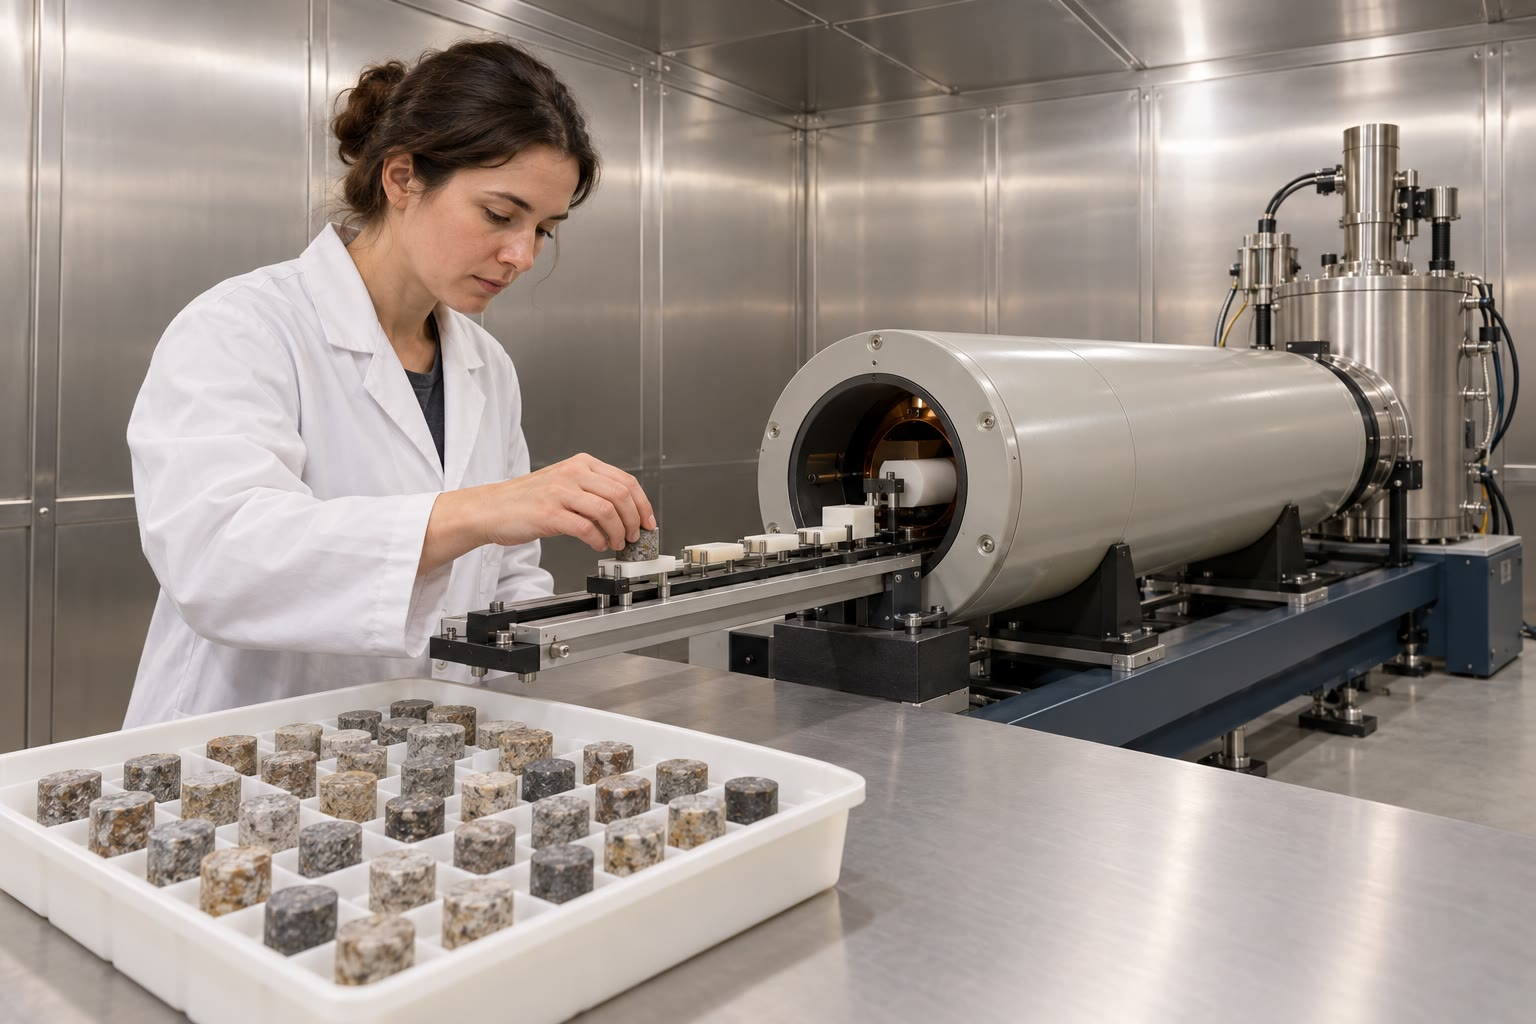
\includegraphics[width=\linewidth]{images/book5/ai/b3-palaeomag-lab.jpg}

{\scriptsize Memuat sampel ke nampan sampel magnetometer di dalam
ruangan terlindung (ilustrasi buatan AI).}
\end{minipage}
\end{inthelab}

\section{Latihan}

\begin{exercise}[$\star$]\label{exo:b3:palaeomagnetism:1}
Dalam medan \omterm{def:b3:palaeomagnetism:main-field}{dipol aksial geosentris}, hitung inklinasi pada lintang
\ang{30}\,LU, dan lintang lokasi tempat inklinasinya \ang{-20}.
\end{exercise}

\begin{exercise}[$\star$]\label{exo:b3:palaeomagnetism:2}
Di suatu stasiun, medan memiliki komponen $X = \qty{20000}{nT}$, $Y =
\qty{-2000}{nT}$ dan $Z = \qty{40000}{nT}$. Hitung $H$, $F$, deklinasi magnetik
dan inklinasi.
\end{exercise}

\begin{exercise}[$\star$]\label{exo:b3:palaeomagnetism:3}
Pada 2025, $g_1^0 = \qty{-29350}{nT}$. Dengan menganggap medan sebagai dipol aksial,
hitung medan di khatulistiwa dan di kutub, serta momen dipol
($a = \qty{6371.2}{km}$, $\mu_0 = 4\pi\times\qty{e-7}{H.m^{-1}}$).
\end{exercise}

\begin{exercise}[$\star$]\label{exo:b3:palaeomagnetism:4}
Sebutkan jenis remanensi yang diperoleh dan kapan ia merekam medan, untuk: (a) aliran
lava yang mendingin; (b) lanau yang mengendap di danau tenang; (c) batu pasir yang
lapisan oksida besinya berubah menjadi hematit selama penguburan awal; (d) basal yang
berada selama satu juta tahun dalam medan saat ini.
\end{exercise}

\begin{exercise}[$\star\star$]\label{exo:b3:palaeomagnetism:5}
Empat sampel dari suatu lokasi memberikan arah $(D, I)$: $(\ang{12}, \ang{48})$,
$(\ang{22}, \ang{44})$, $(\ang{16}, \ang{57})$ dan $(\ang{6}, \ang{53})$.
Hitung vektor satuannya, panjang resultan $R$, arah rata-rata, $k$
dan $\alpha_{95}$.
\end{exercise}

\begin{exercise}[$\star\star$]\label{exo:b3:palaeomagnetism:6}
Suatu lokasi pada \ang{40.0}\,LU, \ang{10.0}\,BT memberikan arah rata-rata $D = \ang{20}$,
$I = \ang{50}$. Hitung \omterm{def:b3:palaeomagnetism:vgp}{paleolintangnya} dan \omterm{def:b3:palaeomagnetism:vgp}{kutub geomagnetik virtualnya}.
\end{exercise}

\begin{exercise}[$\star\star$]\label{exo:b3:palaeomagnetism:7}
IGRF memberikan momen dipol sebesar \qty{8.32e22}{A.m^2} pada 1900 dan
\qty{7.69e22}{A.m^2} pada 2025, dan laju perubahan $g_1^0$ sebesar
\qty{+12.6}{nT/yr} pada 2025. (a) Hitung perubahan relatif momen per
abad. (b) Jika $g_1^0$ mempertahankan laju itu, dalam berapa tahun ia akan mencapai nol?
Mengapa ini bukan sebuah prakiraan?
\end{exercise}

\begin{exercise}[$\star\star$]\label{exo:b3:palaeomagnetism:8}
Remanensi tersisa sebuah sampel, dalam \unit{mA/m} (utara, timur, bawah), adalah
$(32.2, 18.1, 38.2)$ setelah dipanaskan hingga \qty{20}{\celsius}, $(25.8, 18.1, 24.6)$
setelah \qty{300}{\celsius}, dan $(0.0, 0.0, 0.0)$ setelah \qty{580}{\celsius};
\omterm{def:b3:palaeomagnetism:zijderveld}{diagram Zijderveld} lurus di antara setiap pasangan. Hitung arah dan
intensitas komponen yang terlepas antara 20 dan \qty{300}{\celsius} serta yang
terlepas di atas \qty{300}{\celsius}. Yang manakah ChRM, dan apa yang
lainnya?
\end{exercise}

\begin{exercise}[$\star\star$]\label{exo:b3:palaeomagnetism:9}
Suatu formasi memberikan $I = \ang{-35}$ dengan $\alpha_{95} = \ang{5}$. Hitung
\omterm{def:b3:palaeomagnetism:vgp}{paleolintangnya}, rentang \omterm{def:b3:palaeomagnetism:vgp}{paleolintang} yang diizinkan oleh $I \pm \alpha_{95}$,
dan sumbu semi $\mathrm dp$ dan $\mathrm dm$ dari elips kepercayaan
kutubnya.
\end{exercise}

\begin{exercise}[$\star\star\star$]\label{exo:b3:palaeomagnetism:10}
(a) Dari \cref{thm:b3:palaeomagnetism:dipole}, tentukan lintang tempat
inklinasinya \ang{45}, dan rasio medan di kutub terhadap medan di
ekuator. (b) Tunjukkan bahwa $\mathrm dI/\mathrm d\lambda = 2/(1 + 3\sin^2\lambda)$,
dan simpulkan di mana kesalahan inklinasi menghasilkan kesalahan
\omterm{def:b3:palaeomagnetism:vgp}{paleolintang} terbesar. (c) Mengapa \omterm{def:b3:palaeomagnetism:vgp}{paleolintang} dari inklinasi rendah
paling presisi dalam derajat?
\end{exercise}

\begin{exercise}[$\star\star\star$]\label{exo:b3:palaeomagnetism:11}
Suatu situs terletak di \ang{35.0}\,LS, \ang{150.0}\,BT pada lempeng stabil dengan
kutub acuan, untuk umur formasi yang disampel di sana, berada di \ang{70.0}\,LU,
\ang{300.0}\,BT. (a) Hitung jarak sudut $p$ dari situs ke kutub,
inklinasi dan deklinasi yang diharapkan, serta \omterm{def:b3:palaeomagnetism:vgp}{paleolintang} yang diharapkan.
(b) Formasi itu memberikan $D_o = \ang{30.0}$, $I_o = \ang{-60.0}$. Hitung
rotasi $R$ dan perpindahan ke arah kutub $P$, lalu jelaskan maknanya.
\end{exercise}

\begin{exercise}[$\star\star\star$]\label{exo:b3:palaeomagnetism:12}
(a) Dari \cref{prop:b3:palaeomagnetism:fisher}, tunjukkan bahwa peluang
suatu arah berada dalam $\theta$ dari rata-rata adalah $(e^\kappa -
e^{\kappa\cos\theta})/(e^\kappa - e^{-\kappa})$. (b) Untuk $\kappa$ besar dan
$\theta$ kecil, tunjukkan bahwa ini kira-kira $1 - e^{-\kappa\theta^2/2}$, dan simpulkan
bahwa \qty{63}{\percent} dari arah berada dalam $\theta_{63} \approx
\ang{81}/\sqrt\kappa$. (c) Hitung $\theta_{63}$ untuk $\kappa = 50$, dan periksa
\qty{63}{\percent} dengan rumus eksak.
\end{exercise}

\section{Soal: Lapisan merah Kesta}

\begin{problem}[{Soal akhir pekan --- tiga formasi dari sebuah terrane yang berpindah,
arah, kutub, dan rotasinya, serta umur yang termuda}]
\label{pb:b3:palaeomagnetism:1}
% values: calc/ch04.py; palaeomag_stats.py, magnetostratigraphy.py; GPTS: iodp:gpts2004
Kesta adalah terrane rekaan yang kini berada di \ang{47.0}\,LU, \ang{15.0}\,BT, di tepi
benua stabil rekaan. Terrane ini memperlihatkan tiga formasi lapisan merah: A,
\qty{60}{Ma}; B, \qty{30}{Ma}; C, sekitar 3.7 sampai \qty{2.4}{Ma}. Masing-masing
diambil sampelnya di beberapa situs, dan setiap spesimen didemagnetisasi termal;
ChRM dibawa oleh hematit, dan formasi-formasinya horizontal.

\medskip\noindent\textbf{Bagian I --- Arah rata-rata.} Keenam situs formasi A
memberikan $(D, I)$: $(\ang{50}, \ang{37})$, $(\ang{28}, \ang{37})$,
$(\ang{21}, \ang{42})$, $(\ang{24}, \ang{27})$, $(\ang{37}, \ang{39})$,
$(\ang{46}, \ang{38})$.
\begin{enumerate}
  \item Mengapa ChRM yang dibawa hematit dalam lapisan merah dapat lebih muda
        daripada lapisannya? Apa yang akan menunjukkan bahwa ChRM itu tidak jauh lebih muda?
  \item Hitung vektor satuan dari arah pertama.
  \item Keenam vektor satuan berjumlah $(3.8943, 2.6500, 3.5717)$. Hitung $R$ dan
        arah rata-rata formasi A.
  \item Hitung $k$ dan $\alpha_{95}$ untuk formasi A.
  \item Formasi B memberikan, dari 7 situs, $D = \ang{23.9}$, $I = \ang{51.5}$ dan
        $R = 6.8979$; formasi C, dari 8 situs, $D = \ang{3.4}$, $I =
        \ang{63.7}$ dan $R = 7.8707$. Hitung $k$ dan $\alpha_{95}$ masing-masing.
  \item Rata-rata mana yang paling terdefinisi dengan baik, dan formasi mana yang paling baik pengelompokannya?
\end{enumerate}

\medskip\noindent\textbf{Bagian II --- Paleolintang dan kutub.}
\begin{enumerate}[resume]
  \item Hitung \omterm{def:b3:palaeomagnetism:vgp}{paleolintang} formasi A, B, dan C.
  \item Untuk formasi A, hitung paleokolatitud $p$ dan lintang
        \omterm{def:b3:palaeomagnetism:vgp}{kutub geomagnetik virtualnya}.
  \item Hitung bujur kutub itu, dengan memeriksa kasus mana dari
        \cref{thm:b3:palaeomagnetism:pole} yang berlaku.
  \item Hitung $\mathrm dp$ dan $\mathrm dm$ untuk kutub formasi A.
  \item Kutub formasi B dan C berada di \ang{66.5}\,LU, \ang{135.6}\,BT dan
        \ang{87.1}\,LU, \ang{139.1}\,BT. Jelaskan lintasan ketiga kutub
        menurut umur.
\end{enumerate}

\medskip\noindent\textbf{Bagian III --- Umur formasi C.} Pada formasi C,
dari dasarnya, spesimen berpolaritas terbalik sampai \qty{4.2}{m}, normal sampai
\qty{14.8}{m}, terbalik sampai \qty{19.7}{m}, normal sampai \qty{24.6}{m}, terbalik sampai
\qty{29.2}{m} dan normal sampai \qty{54.0}{m}, lalu terbalik hingga puncak pada
\qty{64.0}{m}. Lapisan abu pada \qty{22}{m} diberi penanggalan sekitar \qty{3.2}{Ma}. Subkron
normal dalam kron C2An mencakup 3.596--3.330, 3.207--3.116 dan
3.032--\qty{2.581}{Ma}.
\begin{enumerate}[resume]
  \item Cocokkan zona polaritas dengan skala waktu, dengan menggunakan lapisan abu.
  \item Hitung laju akumulasi antara batas pembalikan pertama dan ketiga,
        dan antara batas pembalikan keempat dan keenam.
  \item Perkirakan umur dasar dan puncak penampang.
  \item Mengapa laju ini merupakan rata-rata selama ratusan ribu tahun, dan apa
        yang dapat membuat laju itu berubah?
\end{enumerate}

\medskip\noindent\textbf{Bagian IV --- Terhadap benua stabil, dan hanyutan.} Kutub acuan
benua stabil berada di \ang{78.0}\,LU, \ang{190.0}\,BT
($A_{95} = \ang{3.0}$) pada \qty{60}{Ma}; \ang{83.5}\,LU, \ang{175.0}\,BT
($\ang{2.5}$) pada \qty{30}{Ma}; dan \ang{87.5}\,LU, \ang{150.0}\,BT ($\ang{2.0}$)
pada \qty{4}{Ma}.
\begin{enumerate}[resume]
  \item Hitung jarak sudut dari Kesta ke kutub acuan
        \qty{60}{Ma}, serta inklinasi dan \omterm{def:b3:palaeomagnetism:vgp}{paleolintang} yang diharapkan.
  \item Hitung deklinasi yang diharapkan pada \qty{60}{Ma}.
  \item Arah yang diharapkan pada 30 dan \qty{4}{Ma} adalah $(\ang{2.9},
        \ang{60.0})$ dan $(\ang{2.5}, \ang{63.6})$. Hitung perpindahan ke arah
        kutub $P$ untuk formasi A, B, dan C.
  \item Hitung rotasi $R$ untuk formasi A, B, dan C.
  \item Hitung kesalahan $\Delta D_o$ dan $\Delta D_x$ untuk formasi A, dan
        kesalahan rotasinya.
  \item Kesalahan $R$ untuk B dan C berturut-turut adalah \ang{13.8} dan \ang{17.9}. Rotasi mana
        yang signifikan pada 95 persen?
  \item Jelaskan sejarah Kesta relatif terhadap benua stabil.
  \item Hitung hanyutan Kesta ke utara sejak formasi A, terhadap
        sumbu rotasi, dalam derajat dan dalam kilometer
        (\qty{111.19}{km} per derajat).
  \item Hitung \omterm{def:b3:palaeomagnetism:vgp}{paleolintang} yang diizinkan oleh $I \pm \alpha_{95}$ untuk
        formasi A, dan ambil satu simpangan baku sebagai separuh lebar interval itu
        dibagi 1.96. Berikan hanyutan Kesta ke utara sejak formasi
        A, dalam kilometer, beserta simpangan bakunya.
\end{enumerate}
\end{problem}
